
%Zeitz auskommentiert\clearpage
%       \begin{center}
% %      \centering
%    %   \begin{wrapfigure}{l}{0.2\textwidth}                    
%  %  \begin{center}
%                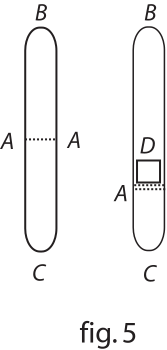
\includegraphics[width=0.2\textwidth]{images/37_3_142v}\\\protect\rule[0cm]{0.5cm}{0cm}\textit{[Fig. 4]}
%                        %\caption{Bildbeschreibung}
%                        \end{center}
 \pstart  Il y a une autre \edtext{Hypothese,}{\lemma{Hypothese}\Bfootnote{Leibniz hat sich insbesondere mit Franciscus Linus\protect\index{Namensregister}{\textso{Linus,} Franciscus 1595\textendash 1675|textit} auseinandergesetzt, der u.~a. auch Gassendi und Pecquet als Repräsentanten dieser Auffassung nennt. Vgl. \textsc{F. Linus}, \cite{00072}\textit{Tractatus de corporum inseparabilitate}, London 1661, S.~9.}} qui attribue l'effect de la suspension dans le vuide\protect\index{Sachverzeichnis}{vide} au ressort de ce peu d'air qui reste dans le recipient. Car, (disent ils,) il est vray que ce ressort est de peu de forces, quand il agit contre un \edtext{autre air,}{\lemma{un}\Afootnote{ \textit{ (1) }\ rien\protect\index{Sachverzeichnis}{rien|textit} \textit{ (2) }\ autre  \textit{(a)}\ ressort, \textit{(b)}\ air, \textit{ L}}} mais \edtext{il est vray aussi qu'}{\lemma{}\Afootnote{il est vray aussi qu' \textit{ erg.} \textit{ L}}} il est d'une force grandissime, et peut estre infinie, quand il agit contre un rien\protect\index{Sachverzeichnis}{rien}; comme donc, le moment que la liqueur ou la placque inferieure se d\'{e}tacheroit, il se feroit un vuide\protect\index{Sachverzeichnis}{vide}, (au moins d'air ou d'autre corps sensible\protect\index{Sachverzeichnis}{corps!sensible})
   % \begin{wrapfigure}{l}{0.2\textwidth}                    
  %  \begin{center}
       %         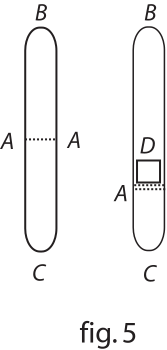
\includegraphics[width=0.2\textwidth]{images/37_3_142v}\\\rule[0cm]{1cm}{0cm}\textit{Fig. 4}
                        %\caption{Bildbeschreibung}
           %             \end{wrapfigure}
                        %@ @ @ Dies ist eine Abstandszeile - fuer den Fall, dass mehrere figures hintereinander kommen, ohne dass dazwischen laengerer Text steht. Dies kann zu einer Fahlermeldung fuehren. @ @ @ \\
                         \edtext{au lieu qu'elle quitte}{\lemma{au}\Afootnote{lieu qu'elle quitte \textit{ erg.} \textit{ L}}}; \edtext{il s'ensuit que le moindre air le pourra empecher, estant capable d'ailleurs de remplir un grandissime espace, quand rien luy resiste: et so\^{u}tenant d\'{e}ja en effect par son ressort}{\lemma{quitte;}\Afootnote{ \textit{ (1) }\  par consequent le moindre   \textbar\ air \textit{ erg.}\ \textbar\   \textit{(a)}\ sera capable de l'empecher \textit{(b)}\ le pourra empecher. \textit{ (2) }\  Ils adjoustent que la moindre bulle d'air seroit capable de remplir un espace grandissime;  \textit{(a)}\ et que le moindre bulle  \textit{(aa)}\ so\^{u}tient \textit{(bb)}\ est capable en effect de \textit{(b)}\ et so\^{u}tient en effect \textit{ (3) }\ il [...] ressort \textit{ L}}} l'effort de toute l'atmosphere\protect\index{Sachverzeichnis}{atmosph\`{e}re}, qui le presse. \edtext{Car il est constant qu'une petite bulle d'air ordinaire ne peut estre press\'{e}e d'avantage par tout le reste de la Masse d'air, autrement ce seroit d\'{e}ja fait.}{\lemma{}\Afootnote{Car [...] autrement \textit{ (1) }\ elle l'auroit d\'{e}ja fait \textit{ (2) }\ ce seroit d\'{e}ja fait. \textit{ erg.} \textit{ L}}}
                                             %@ @ @ Dies ist eine Abstandszeile - fuer den Fall, dass mehrere figures hintereinander kommen, ohne dass dazwischen laengerer Text steht. Dies kann zu einer Fahlermeldung fuehren. @ @ @ \\
                          Par consequent si dans la \textso{fig. 5.} 
                     l'espace \textit{BD} estoit vuide d'air ou d'autre corps sensible\protect\index{Sachverzeichnis}{corps!sensible}, le peu d'air \textit{AC} seroit capable, (si nous le croyons, \edtext{sur leur parole}{\lemma{}\Afootnote{sur leur parole \textit{ erg.} \textit{ L}}}) d'elever le poids\protect\index{Sachverzeichnis}{poids} \textit{D} jusqu'\`{a} \textit{B} de quelque grandeur que ce poids\protect\index{Sachverzeichnis}{poids} puisse estre. Mais voila comme je crois pouuoir demonstrer le contraire: Soit le Tuyau \textit{AA} plein d'air uniforme \textit{AB}, et \textit{AC}; et puis l'air \textit{AC} soit press\'{e} par le poids\protect\index{Sachverzeichnis}{poids} \textit{D} dans l'espace \textit{DB} \edtext{qui est la}{\lemma{}\Afootnote{qui est la \textit{ erg.} \textit{ L}}} moiti\'{e} de l'espace \textit{AC} perdant la moiti\'{e} de son volume. Il est manifeste que le poids \textit{D} avec l'air \textit{BA} qui occupe \`{a} present un espace plus grand \textit{DB} fait la m\^{e}me chose \edtext{contre l'air \textit{AC}, \`{a} present en \textit{DC}}{\lemma{}\Afootnote{contre l'air   \textbar\ \textit{AC}, \`{a} present \textit{ erg.}\ \textbar\  en \textit{DC} \textit{ erg.} \textit{ L}}} que feroit l'air qui est en \textit{DB} s'il estoit aussi condens\'{e} que l'air en \textit{DC} c'est \`{a} dire s'il le   contraindroit ou retiendroit en \textit{DC} \`{a} cause de leur \edtext{uniformit\'{e}. Donc}{\lemma{uniformit\'{e}.}\Afootnote{ \textit{ (1) }\ Ergo \textit{ (2) }\ Donc \textit{ L}}} le poids \textit{D} \edtext{(+) plus la force de l'air \textit{BA} en \textit{DB} (=) \'{e}galeroit la force de l'air \textit{AB} en \textit{DB}}{\lemma{\textit{D}}\Afootnote{ \textit{ (1) }\ + l'air \textit{BA} = l'air en \textit{DB} \textit{ (2) }\ (+) [...] \textit{DB} \textit{ L}}} si sa condensation \edtext{seroit suppos\'{e}e}{\lemma{condensation}\Afootnote{ \textit{ (1) }\ est \textit{ (2) }\ seroit suppos\'{e}e \textit{ L}}} \'{e}galle \`{a} celle de l'air \edtext{\textit{AC} en \textit{DC}.}{\lemma{l'air}\Afootnote{ \textit{ (1) }\ en \textit{DC} \textit{ (2) }\ \textit{AC} en \textit{DC}. \textit{ L}}} Or l'air \textit{BA} en \textit{DB} \'{e}galle (=) l'air \textit{AC} en \textit{DC} mais \edtext{\textit{BD}}{\lemma{}\Afootnote{\textit{BD} \textit{ erg.} \textit{ L}}} le volume de l'air \textit{BA}, en \textit{DB} est \`{a} \textit{DC} volume de l'air \textit{AC} en \textit{DC}, comme 3. \`{a} 1. Donc la condensation de l'air \textit{AC} en \textit{DC} est tripl\'{e} de l'air \textit{BA} en \textit{DB}. Par consequent si l'air \textit{BA} en \textit{DB} doit estre d'une consistence \'{e}gale \`{a} l'air \textit{AC} en \textit{DC} il faut qu'il soit tripl\'{e}. Par consequent le poids \edtext{\textit{D}}{\lemma{\textit{D}}\Afootnote{ \textit{ erg.} \textit{ L}}} + \edtext{la force de l'air \textit{BA} en \textit{DB} = la force de l'air \textit{AB} en \textit{DB} mais tripl\'{e} = la force de l'air \textit{AC} en \textit{DC}.}{\lemma{+}\Afootnote{ \textit{ (1) }\ l'air \textit{BA} en \textit{DB} = l'air \textit{AB} en \textit{DB}   \textbar\ mais tripl\'{e} = l'air \textit{AC} en \textit{DC} \textit{ erg.}\ \textbar\  \textit{ (2) }\ la [...] \textit{DC}. \textit{ L}}} Donc le poids \textit{D} \'{e}gale deux tiers de la force de l'air \textit{AC} en \textit{DC}. Donc $\displaystyle\frac{3}{2}D=\rule[-4mm]{0mm}{10mm}$%@@@ G R A F I K @@@% \begin{wrapfigure}{l}{0.4\textwidth}                    
                %\includegraphics[width=0.4\textwidth]{../images/Recherche+de+la+raison+de+ces+ph%26eacute%3Bnom%26egrave%3Bnes+avec+des+exp%26eacute%3Briences+projett%26eacute%3Bes+pour+s%27en+%26eacute%3Bclaircir+d%27avantage%3B+et+une+hypoth%26egrave%3Bse+nouvelle/LH037%2C03_142v/files/100481.png}
                        %\caption{Bildbeschreibung}
                        %\end{wrapfigure}
                        %@ @ @ Dies ist eine Abstandszeile - fuer den Fall, dass mehrere figures hintereinander kommen, ohne dass dazwischen laengerer Text steht. Dies kann zu einer Fahlermeldung fuehren. @ @ @ \\
                     la force de l'air \textit{AC} en \textit{DC} et par consequent si l'on augmente le poids \textit{D} de sa moiti\'{e}, il so\^{u}tiendra le ressort de l'air \textit{AC} en \textit{DC} quoyque l'air en \textit{BD} n'y contribue rien, et quoyque l'espace \textit{BD} soit vuide.
                     \pend 
                     